\section{Introducción}
\begin{frame}{Qubits}
    \begin{columns}
        \begin{column}{0.5\textwidth}
            Sistemas cuánticos de dos niveles:\pause
            \begin{equation}
                \ket{\psi}=\alpha\ket{0}+\beta\ket{1}.\nonumber
            \end{equation}\pause
            Reescribible como:\pause
            \begin{equation}
                \ket{\psi}=\cos(\frac{\theta}{2})\ket{0}+e^{\rmi\varphi}\sin(\frac{\theta}{2})\ket{1}.\nonumber
            \end{equation}
        \end{column}
        \pause
        \begin{column}{0.5\textwidth}
            \centering
            \BlochSphere
        \end{column}
    \end{columns}
\end{frame}

%###########################
%# Descripciones efectivas #
\begin{frame}{Dinámica que emerge de una descripción efectiva: motivación}
    \begin{center}
        ``Dinámica \textbf{efectiva} de un sistema de N qubits''
    \end{center}
    \pause
    \begin{columns}
        \begin{column}{0.5\textwidth}
            \begin{center}
                Dinámica \textbf{efectiva}\\
                \pause
                $\downarrow$\\
                Dinámica {\tiny(que emerge de una descripción)} \textbf{efectiva}\mycite{CGEmergingDynamics}
            \end{center}
            \pause
            Aquí, 
            \begin{center}
                \textit{efectiva}$\iff$\textit{gruesa}.
            \end{center}
        \end{column}
        \pause
        \begin{column}{0.5\textwidth}
            Una descripción de grano grueso de un sistema es resultado de\pause
            \begin{itemize}
                \item Aparato de medición imperfecto
                \item Descarte de grados de libertad del sistema
            \end{itemize}
        \end{column}
    \end{columns}
    \pause
    \begin{center}
        \begin{tcolorbox}
            \begin{center}
                Un modelo de grano grueso permite estudiar la emergencia de comportamientos comúnmente física clásica
            \end{center}
        \end{tcolorbox}
    \end{center}
\end{frame}
%###########################


%###########################
% ## Operador de densidad ##
\subsection{El operador de densidad}

\begin{frame}{Mezclas estadísticas}
    \begin{columns}
        \begin{column}{0.5\textwidth}
            \begin{block}{Probabilidad cuántica}
            Los vectores de estado contienen probabilidad cuántica:
            \begin{equation}
                \ket{\psi}=\alpha\ket{0}+\beta\ket{1},\nonumber
            \end{equation}
            \pause
            de la que se recupera la regla de Born:
            \begin{equation}
                p(\ket{0})=\abs{\alpha}^{2}\qquad p(\ket{1})=\abs{\beta}^{2}\nonumber
            \end{equation}
        \end{block}
        \end{column}
        \pause
        \begin{column}{0.5\textwidth}
            \begin{block}{Probabilidad \textit{por ignorancia}}
            Un sistema del que se sabe se halla en el estado $\ket{\varphi_{j}}$ con probabilidad $p_{j}$.\\
            \vspace{0.2cm}
            \pause
            De este sistema se halla en un estado de \textit{mezcla estadística}.\\
            \vspace{0.2cm}
            \pause
            Es descrito por el operador de densidad
            \begin{equation}
                \rho=\sum_{j}p_{j}\dyad{\varphi_{j}}.\nonumber
            \end{equation}
        \end{block}
        \end{column}
    \end{columns}
\end{frame}
\begin{frame}{Parametrización}
    \begin{columns}
        \begin{column}{0.5\textwidth}
            Parametrizar usando producto punto\mycite{Chuang}
            \begin{equation}
                \rho=\frac{1}{2}\qty(\Id_{2}\Tr(\rho)+\sum_{k=1}^{3}\Tr(\rho\pauli{k})\pauli{k}).\nonumber
            \end{equation}
            \pause
            El vector de Bloch es
            \begin{equation}
                \vec{r}_{\rho}=\begin{pmatrix}
                    \Tr(\rho\pauli{x})\\
                    \Tr(\rho\pauli{y})\\
                    \Tr(\rho\pauli{z})
                \end{pmatrix}\nonumber
            \end{equation}
        \end{column}
        \pause
        \begin{column}{0.5\textwidth}
            \centering
            \BlochSphereDensity
        \end{column}
    \end{columns}
\end{frame}
%###########################


%###########################
%#### Sistemas abiertos ####
\begin{frame}{Sistemas multipartitos y canales cuánticos}
    \begin{columns}
        \begin{column}{0.5\textwidth}
            \begin{block}{Combinar y reducir}
                \begin{center}
            Si $\rho_{\text{bi}}$ describe dos qubits A y B,\pause \\
            $\hilbert_{\text{bi}}=\hilbert_{2}\otimes\hilbert_{2}$. \pause \\
            \vspace{0.2cm}
           ¿Y si es relevante \textbf{una} partícula?\pause \\
            $\rho^{A}=\Tr_{B}(\rho_{\text{bi}})$. \pause \\
            \vspace{0.2cm} 
            Sistema multipartito $\rightarrow$ von Neumann\\
            $\rmi\hbar\frac{d}{d t} \rho_{\text{bi}}(t)=[H,\rho_{\text{bi}}(t)]$. \pause \\
            \vspace{0.2cm}
            Trazando:\\
            $\rmi\hbar\frac{d}{d t} \rho^{A}(t)=\Tr_{B}([H,\rho_{\text{bi}}(t)])$.\pause \\
                \end{center}
            \end{block}
        \end{column}
        \pause
        \begin{column}{0.5\textwidth}
        \begin{block}{Canales cuánticos}
            \begin{itemize}
                \item Son generalización lineal de la dinámica unitaria: $\mcE_{t}$.\pause
                \item Modelan procesos ruidosos.\pause
                \item Relacionados a sistemas abiertos.\pause
                \item Tienen representación en operadores de \textbf{Kraus}\mycite{Breuer}:
                    \begin{align}
                        \mcE(\rho)=\sum_{k}A_{k}\rho A^{\dagger}_{k},& &\sum_{k}A_{k}^{\dagger}A_{k}=\Id \nonumber
                    \end{align}
            \end{itemize}
        \end{block}
        \end{column}
    \end{columns}
\end{frame}
%###########################



%###########################
%### Ejemplos de canales ###
\begin{frame}{Ejemplo de canal cuántico: desfasamiento}
    \begin{center}
        El \textit{canal de desfasamiento} tiene operadores de Kraus $\{\sqrt{p}\Id,\sqrt{(1-p)}\pauli{3}\}$.
    \end{center}
    \begin{figure}
        \centering
        \begin{subfigure}{0.45\textwidth}
            \centering
            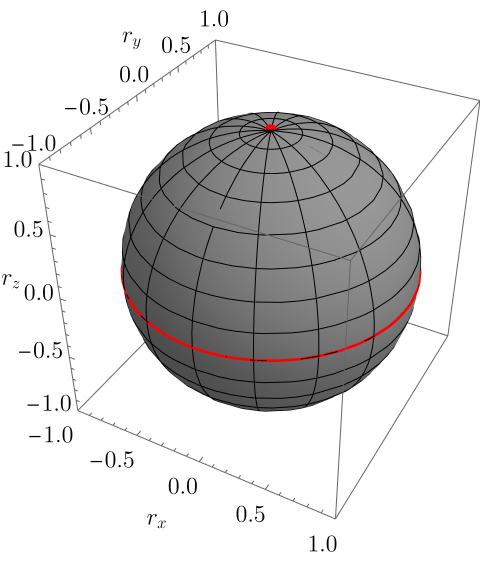
\includegraphics[width=0.5\textwidth]{figures/whole_sphere.png}
        \end{subfigure}
        \begin{subfigure}{0.45\textwidth}
            \centering
            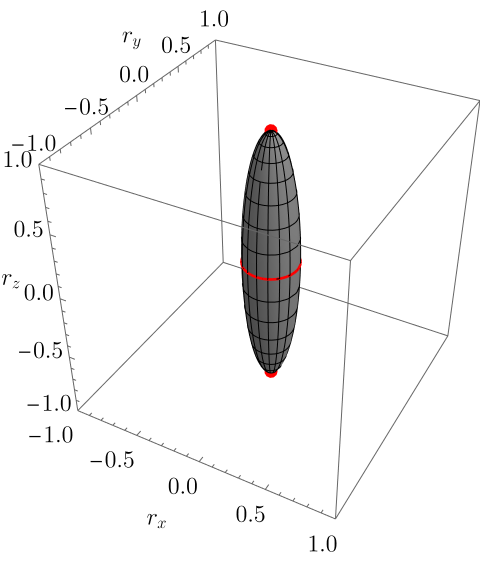
\includegraphics[width=0.5\textwidth]{figures/dephased.png}
        \end{subfigure}
        \caption{Efecto del canal de desfasamiento sobre la esfera de Bloch si $p=0.6$}
    \end{figure}
\end{frame}
\begin{frame}{Ejemplo de canal cuántico: bitflip}
    \begin{center}
        El \textit{canal de bitflip} tiene operadores de Kraus $\{\sqrt{p}\Id,\sqrt{(1-p)}\pauli{1}\}$.
    \end{center}
    \begin{figure}
        \centering
        \begin{subfigure}{0.45\textwidth}
            \centering
            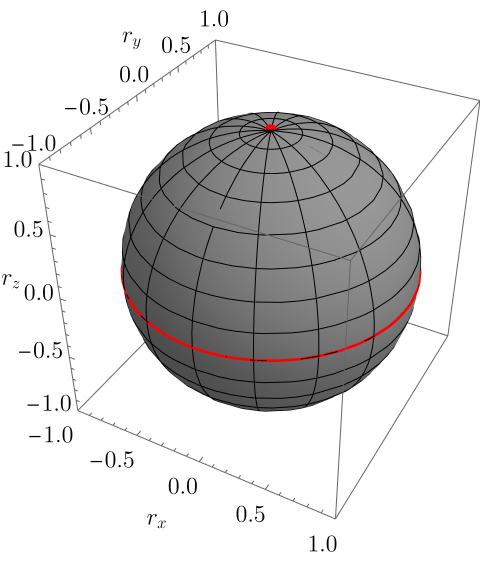
\includegraphics[width=0.5\textwidth]{figures/whole_sphere.png}
        \end{subfigure}
        \begin{subfigure}{0.45\textwidth}
            \centering
            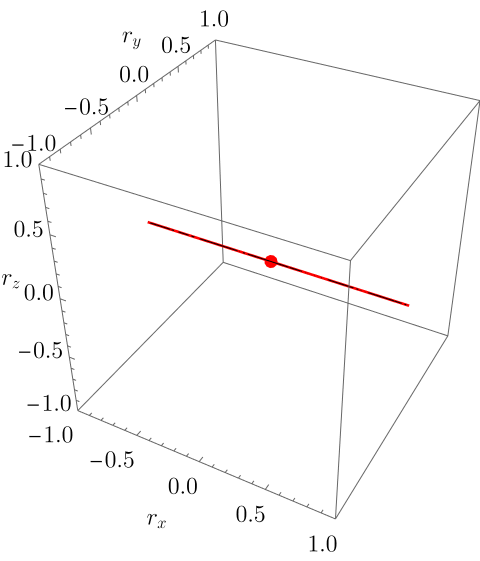
\includegraphics[width=0.5\textwidth]{figures/bitflip.png}
        \end{subfigure}
        \caption{Efecto del canal de bit flip sobre la esfera de Bloch si $p=0.5$}
    \end{figure}
\end{frame}
\begin{frame}{Ejemplo de canal cuántico: despolarización}
    Finalmente, el \textit{canal de despolarización} se define mediante
    \begin{equation}
        \rho\mapsto p\frac{1}{2}\Id+(1-p)\rho\nonumber.
    \end{equation}
    \begin{figure}
        \centering
        \begin{subfigure}{0.45\textwidth}
            \centering
            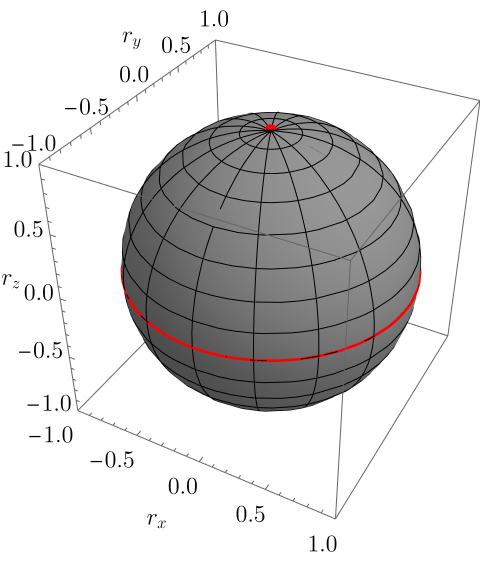
\includegraphics[width=0.5\textwidth]{figures/whole_sphere.png}
        \end{subfigure}
        \begin{subfigure}{0.45\textwidth}
            \centering
            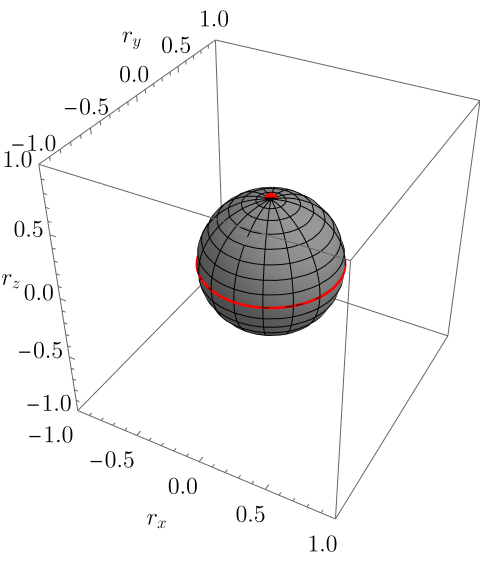
\includegraphics[width=0.5\textwidth]{figures/depol.png}
        \end{subfigure}
        \caption{Efecto del canal de despolarización sobre la esfera de Bloch si $p=0.6$}
    \end{figure}
\end{frame}
%###########################

\begin{frame}{Planteamiento del problema}
    \begin{center}
        Se estudia la dinámica que emerge de una descripción efectiva ${\color{blue}\mcC}$. \pause
    \end{center}
    \begin{columns}
        \begin{column}{0.5\textwidth}
            \begin{center}
                $$\begin{tikzpicture}[node distance=2cm, auto]
                    \draw [blue,fill=cyan!20, fill opacity=0.6] (1.2cm,0cm) ellipse (2.2cm and 0.7cm);
                    \draw [red,fill=red!20, fill opacity=0.5] (1.2cm,-1.8cm) ellipse (2.2cm and 0.7cm);
                    \node (ef0) {$\rho_{\ef}(0)$};
                    \node (eft) [right=1.5cm of ef0] {$\rho_{\ef}(t)$};
                    \node (varrho0) [below=1.2cm of ef0] {$\varrho_{\text{\textcolor{red}{?}}}(0)$};
                    \node (varrhot) [below=1.2cm of eft] {$\varrho_{\text{\textcolor{red}{?}}}(t)$};
                    \draw[->] (ef0) to node {\textbf{?}} (eft);
                    \draw[->] (varrho0) to node [swap] {$\mcE_{t}$} 
                    (varrhot);
                    \draw[blue,->] (varrho0) to node [left] {$\mcC$} 
                    (ef0);
                    \draw[blue,->] (varrhot) to node [right] {$\mcC$} 
                    (eft);
                  \end{tikzpicture}$$
            \end{center}
        \end{column}
        \pause
        \begin{column}{0.5\textwidth}
            \begin{center}
                $$\begin{tikzpicture}[node distance=2cm, auto]
                    \draw [blue,fill=cyan!20, fill opacity=0.6] (1.2cm,0cm) ellipse (2.2cm and 0.7cm);
                    \draw [red,fill=red!20, fill opacity=0.5] (1.2cm,-1.8cm) ellipse (2.2cm and 0.7cm);
                    \node (ef0) {$\rho_{\ef}(0)$};
                    \node (eft) [right=1.5cm of ef0] {$\rho_{\ef}(t)$};
                    \node (varrho0) [below=1.2cm of ef0] {$\varrho_{\text{\textcolor{red}{?}}}(0)$};
                    \node (varrhot) [below=1.2cm of eft] {$\varrho_{\text{\textcolor{red}{?}}}(t)$};
                    \draw[->] (ef0) to node {\textbf{?}} (eft);
                    \draw[->] (varrho0) to node [swap] {$\mcE_{t}$} 
                    (varrhot);
                    \draw[red,->] (ef0) to node [left] {$\mcA$} 
                    (varrho0);
                    \draw[blue,->] (varrhot) to node [right] {$\mcC$} 
                    (eft);
                  \end{tikzpicture}$$
            \end{center}
              \pause
        \end{column}
    \end{columns}
    \begin{center}
        ¿Cómo construir ${\color{red}\mcA}$?
    \end{center}
\end{frame}

%###########################
%#### Entropía y MaxEnt ####
\subsection{Entropía e información}

\begin{frame}{Entropía en teoría de información clásica}
    \begin{columns}
        \begin{column}{0.5\textwidth}
            \begin{block}{Información clásica}
            \begin{center}
                A cada evento se le puede asociar una cantidad de información\pause
            \end{center}
            \begin{itemize}
                \item ``Número entre 1 y 6''$\rightarrow$ no da información. \pause
                \item ``No cayó 6''$\rightarrow$ poca información\pause
                \item ``Cayó 5''$\rightarrow$ más información\pause
            \end{itemize}
            Entonces $\text{información}\propto f\qty(p(\text{evento})^{-1})$
        \end{block}
        \end{column}
        \pause
        \begin{column}{0.5\textwidth}
            \begin{block}{Entropía de Shannon}
            Claude Shannon demostró\mycite{Shannon}
            \begin{equation}
                S_{\text{S}}=-k\sum_{j}p(x_{j})\log{p(x_{j})}.\nonumber
            \end{equation}\pause
            La \textit{entropía de Shannon} representa la información promedio.
        \end{block}
        \end{column}
    \end{columns}
\end{frame}

\subsection{El Principio de Máxima Entropía}

\begin{frame}{Intuición y enunciación del Principio de Máxima Entropía}
    \begin{columns}
        \begin{column}{0.5\textwidth}
            \begin{block}{Usando dados: {\usefont{U}{dice3d}{m}{n}6a 2b 3d}}
                \pauses
                \begin{center}   
                Supóngase que $\expval{\text{\Pisymbol{dice3d}{102}}}=3.5$\\ \pause
                ¿$p(x)$?\\ \pause
                Dado balanceado:
                \begin{tabular}{ c c c }
                    $p(\epsdice{1})=\frac{1}{6}$ & $p(\epsdice{2})=\frac{1}{6}$ & $p(\epsdice{3})=\frac{1}{6}$ \\
                    $p(\epsdice{4})=\frac{1}{6}$ & $p(\epsdice{5})=\frac{1}{6}$ & $p(\epsdice{6})=\frac{1}{6}$
                \end{tabular}\pause \\
                \vspace{0.3cm}
                Dado pesado:
                \begin{tabular}{ c c c }
                    $p(\epsdice{5})=\frac{1}{2}$ & $p(\epsdice{2})=\frac{1}{2}$ & $p(\epsdice{1})=0$ \\
                    $p(\epsdice{3})=0$ & $p(\epsdice{4})=0$ & $p(\epsdice{6})=0$
                \end{tabular}
                \end{center}
            \end{block}
        \end{column}
        \pause
        \begin{column}{0.5\textwidth}
            \begin{block}{El principio de Máxima Entropía}
                ``La distribución de probabilidad que maximiza la entropía es la única asignación sin sesgo. Cualquier otra implicaría la suposición arbitraria de información que no se tiene''.\mycite{JaynesI}
            \end{block}
            El principio de máxima entropía fue introducido por E. T. Jaynes en 1957. \pause
        \end{column}
    \end{columns}
\end{frame}
\begin{frame}{El Principio de Máxima Entropía clásico}
    Sean $x_{j}$ los valores de $X$, $\expval{f_{l}(x)}$ conocidos. Maximizamos la entropía:\pause
    \begin{equation}
        \mcL=-S_{\text{S}}(p)\pause+\sum_{l}\lambda_{l}\qty(\sum_{j}p(x_{j})f_{l}(x_{j})-\expval{f_{l}(x)})\pause+\mu\qty(\sum_{j}p(x_{j})-1).\nonumber
    \end{equation}\pause
    Resolviendo: \pause
    \begin{equation}
        p(x_{j})=\frac{1}{Z}\exp[-\frac{1}{k}\sum_{l}\lambda_{l}f_{l}(x_{j})].\nonumber
    \end{equation}
\end{frame}
\begin{frame}{El Principio de Máxima Entropía cuántico}
    Usamos la entropía de von Neuman \pause 
    \begin{equation}
        S=-Tr(\rho\ln(\rho))\nonumber
    \end{equation}\pause
    y asumimos que conocemos $\expval{A_{k}}$
    \begin{equation}
        S_{\text{N}}=-Tr(\rho\ln(\rho))\pause\xrightarrow{\text{maximización}}\rho=\frac{1}{Z}e^{-\sum_{k}\lambda_{k} A_{k}}\nonumber
    \end{equation}\pause
    Así que el operador de densidad que maximiza la entropía\mycite{JaynesII}\mycite{FormalJaynes}:
    \begin{center}
        \tcbox{$\rho=\frac{1}{Z}e^{-\sum_{k}\lambda_{k} A_{k}}$}
    \end{center}
\end{frame}
%###########################


%###########################
%###########################
\begin{frame}{El problema}
    \begin{center}
        ``Dinámica efectiva de un sistema de N qubits\\
        Utilizando el Principio de Máxima Entropía''
        $$\begin{tikzpicture}[node distance=2cm, auto]
            \draw [blue,fill=cyan!20, fill opacity=0.6] (1.2cm,0cm) ellipse (2.2cm and 0.7cm);
            \draw [red,fill=red!20, fill opacity=0.5] (1.2cm,-1.8cm) ellipse (2.2cm and 0.7cm);
            \node (ef0) {$\rho_{\ef}(0)$};
            \node (eft) [right=1.5cm of ef0] {$\rho_{\ef}(t)$};
            \node (varrho0) [below=1.2cm of ef0] {$\varrho_{\max}(0)$};
            \node (varrhot) [below=1.2cm of eft] {$\varrho_{\max}(t)$};
            \draw[->] (ef0) to node {$\Gamma_{t}$} (eft);
            \draw[->] (varrho0) to node [swap] {$\mcE_{t}$} 
            (varrhot);
            \draw[red,->] (ef0) to node [left] {$\mcA_{\mcC}^{\max}$} 
            (varrho0);
            \draw[blue,->] (varrhot) to node [right] {$\mcC$} 
            (eft);
          \end{tikzpicture}$$ \pause
          Queda construir matemáticamente $\color{blue}\mcC$ y $\color{red}\mcA_{\mcC}^{\max}$.
    \end{center}
\end{frame}
%###########################